\documentclass[10pt]{article}
	\usepackage[utf8]{inputenc}
	\usepackage[onehalfspacing]{setspace}
	\usepackage{enumitem}
	\usepackage{varwidth}
  \usepackage{graphicx}
  \usepackage{listings}
  \usepackage{color}
	\usepackage{geometry}
	\usepackage{lscape}
	\usepackage{pgfgantt} % Gantt chart
  \usepackage{textcomp} % \texttrademark
  \usepackage{multicol}
  \usepackage{lipsum}% dummy text
  \usepackage{tikz, wasysym}
  \usetikzlibrary{shapes.multipart}
  \usetikzlibrary{automata,positioning}
	\PassOptionsToPackage{hyphens}{url}\usepackage{hyperref}
	\usepackage{hyperref}
  \setlist{nosep, after=\vspace{\baselineskip}}
  \setlength{\columnseprule}{0pt}
  \graphicspath{ {images/} }

  \lstset{language=python,
  frame=single,
  basicstyle=\footnotesize\ttfamily,
  captionpos=b,
  tabsize=2,
  }

\begin{document}

%%%%%%%%%%%%%%%%%%%%%%%%%%%%%%%%%%% /TITLE PAGE %%%%%%%%%%%%%%%%%%%%%%%%%%%%%%%%
\begin{titlepage}
	\centering
  % \vspace{1cm}
  {\scshape\Large USI\par}
	{\scshape\Large Theory of Computation\par}
	\vspace{1.5cm}
	{\huge\bfseries SAT Lab\par}\vspace{0.5cm}
	{\large\bfseries Practical Homework 2\par}
	\vspace{2cm}
	{\Large Andrea Frachini, Davide Bucher, Lorenzo Spoleti, Milo Wroblewski, Samuele Bischof\par}

\end{titlepage}
%%%%%%%%%%%%%%%%%%%%%%%%%%%%%%%%%%% TITLE PAGE/ %%%%%%%%%%%%%%%%%%%%%%%%%%%%%%%%


\section*{Sudoku}
The application is bundled inside an Electron application.
The user can play sudoku on the board, when the solve button is pressed,
electron writes the
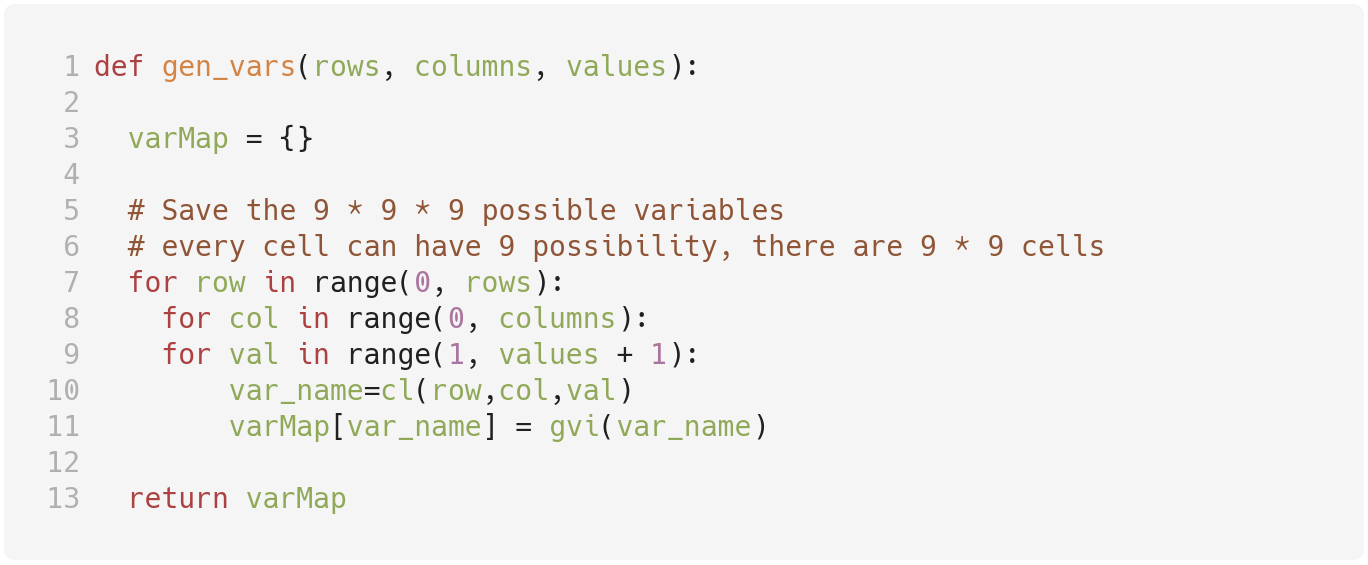
\includegraphics[width=\linewidth]{genVars.png}
This function generates the variables. It works

\end{document}